\documentclass[11pt,a4paper,onecolumn]{report}
\usepackage{amsmath}
\usepackage{mathtools}
\usepackage{lmodern}
\DeclarePairedDelimiter{\abs}{\lvert}{\rvert}
\usepackage{bm}
\usepackage[margin=2cm]{geometry}
\usepackage{array}
\usepackage{physics}
\usepackage{amssymb}
\usepackage{textcomp}
\usepackage[T1]{fontenc}
\usepackage{gensymb}
\usepackage{graphicx}
\usepackage{fancyhdr}
\pagestyle{fancy}
\setlength{\headheight}{13.6pt}

\usepackage{tikz}
\usetikzlibrary{shapes.geometric, arrows, calc}
\usepackage[nottoc, numbib]{tocbibind}
\tikzstyle{cool} = [rectangle, rounded corners, minimum width=3cm, minimum
height=1cm, text centered, draw=black, fill=gray!30, text width=3cm]
\tikzstyle{arrow} = [thick, ->, >=stealth] \tikzstyle{line} = [thick, -,
>=stealth]

\usepackage[detect-all]{siunitx}
\usepackage{breqn}
\usepackage{subfigure}
\usepackage{geometry}
\usepackage{listings}
\usepackage{caption}
\usepackage[utf8]{inputenc}
\usepackage{hyperref}
\usepackage{titlesec}
\usepackage[square,numbers,comma,sort&compress]{natbib}
\usepackage{upgreek}
\usepackage{aas_macros}
\usepackage{doi}
\usepackage{siunitx}
\usepackage{textgreek}


\geometry{a4paper, left=25mm, top=25mm,} % total={160mm,247mm} <- overspecification
\graphicspath{{figures/} }
\renewcommand{\listfigurename}{Figures}


\captionsetup{justification   = raggedright, singlelinecheck = false}

\hypersetup{colorlinks, citecolor=black, filecolor=black, linkcolor=black,
    urlcolor=black}

\renewcommand{\bibname}{References}

\bibpunct{(}{)}{;}{a}{}{,}

\hypersetup{colorlinks, citecolor=black, filecolor=black, linkcolor=black,
    urlcolor=black}


\newcommand*\chem[1]{\ensuremath{\mathrm{#1}}}

\newcommand{\threevdots}{%
  \vbox{\baselineskip1ex\lineskiplimit0pt%
  \hbox{.}\hbox{.}\hbox{.}}}



% diagnose: Label(s) may have changed. Rerun to get cross-references right.
% \def\@testdef #1#2#3{% \def\reserved@a{#3}\expandafter \ifx \csname
% #1@#2\endcsname \reserved@a  \else \typeout{^^Jlabel #2 changed:^^J%
% \meaning\reserved@a^^J% \expandafter\meaning\csname #1@#2\endcsname^^J}%
% \@tempswatrue \fi}


%opening
\title{Thesis}
\author{Cameron Smith\\
Student ID: 28792912\\
Supervisors: Andrew Casey, Alina Donea}
\date{\today}



\begin{document}


\begin{titlepage}
  \begin{center}
    \vspace*{2cm}
    \Huge
    \textbf{Title of your Thesis}

    \vspace{2cm}
    \LARGE
    \textbf{Cameron Smith}

    \vspace{0.8cm}
    \Large \textit{Supervisors:}\\
    Andrew Casey\\
    Alina Donea

    \vfill
    \large
    An honours thesis presented for the degree of\\
    Bachelor of Science Advanced - Research (Honours)

    \vspace{0.3cm}
    \includegraphics[width=0.2\linewidth]{"Monash_Logo"}\\
    School of Physics and Astronomy\\
    Faculty of Science\\
    Monash University\\
    Australia

    \vspace{0.5cm}

    \today

  \end{center}
\end{titlepage}

\chapter*{Abstract}



\chapter*{Acknowledgements}

\tableofcontents


\listoffigures







%
%
%
%
\chapter{Introduction}
%
%
%
%



%TODO: Introduction (maybe borrow slightly from lit review)


%
% Project outline from lit review
%

To train a cGAN to generate magnetograms from seismic maps, we require a
training set consisting of seismic maps and the corresponding magnetograms.
While the farside seismic maps are readily available\footnote{See
  \url{http://jsoc.stanford.edu/data/farside/}.}, corresponding magnetograms are
not. However, not all hope is lost. The STEREO-A spacecraft is in a heliocentric
orbit that traverses the Sun relative to the Earth, allowing it to observe the
farside during some points of the orbit. While STEREO-A does not capture
magnetograms of the Sun, it does take EUV images which can be used to create
magnetograms by using a cGAN \citep{Kim2019}.\\

A small complication is that no data is available from when STEREO-A was
directly opposite the Earth (between March and July 2015), due to the
interference from the Sun. This limits the ability to get magnetograms that
exactly coincide with the farside seismic maps. To compensate for this, we can
match farside seismic maps with images taken by STEREO-A at an earlier (later)
time when it is behind (ahead of) the farside, such that the same `face' of the
Sun is imaged due to it's rotation. After generating the magnetograms from the
STEREO-A EUV images, we can create a dataset of seismic maps with the
corresponding magnetogram (albeit with some time difference). This process is
summarised in Figure \ref{fig:Project_summary}.\\



\begin{figure}
  \centering
  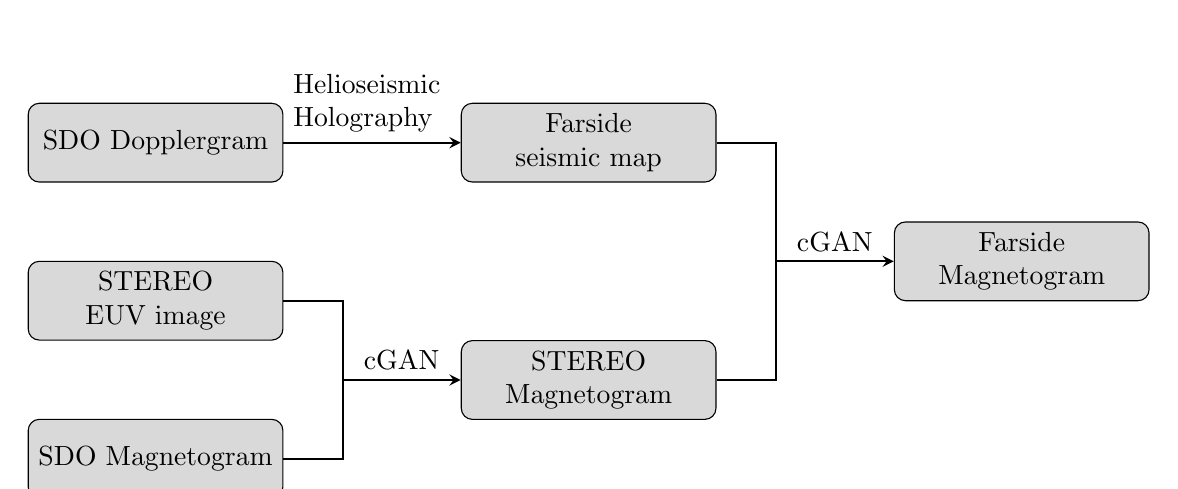
\begin{tikzpicture}[node distance=5.5cm]
    % \draw[help lines] (0,-5) grid (10,10);
    \node (D) [cool, above=1.5cm] {SDO Dopplergram}; \node (P) [cool, right
      of=D] {Farside \quad \quad \quad \qquad  seismic map}; \node (E) [cool]
    {STEREO EUV image}; \node (M) [cool, right of=E, below=0.5cm] {STEREO
      Magnetogram}; \node (F) [cool, right of=M, above=1cm] {Farside\\
      Magnetogram}; \node (S) [cool, below=1.5cm] {SDO Magnetogram};

    \coordinate (FF) at ([xshift=-1.5cm]F.west); % we collect the edges in
    front of Q
    \coordinate (MM) at ([xshift=-1.5cm]M.west); % we collect the edges in
    front of Q

    \draw [arrow] (D) -- node[anchor=south, text width=2cm] {Helioseismic
      Holography} (P); \draw [arrow] (MM) -- node[anchor=south] {cGAN} (M);
    \draw [line] (P) -|  (FF); \draw [line] (M) -|  (FF); \draw [line] (S) -|
    (MM); \draw [line] (E) -|  (MM); \draw [arrow] (FF) -- node[anchor=south]
    {cGAN} (F);

  \end{tikzpicture}
  \caption[Project Pipeline]{Summary of the project. A cGAN is trained on SDO
    data to be able to generate EUV images. This is applied to STEREO EUV images
    to generate STEREO magnetograms. These are used in conjunction with farside
    seismic maps to train a new cGAN to generate magnetograms from seismic maps,
    allowing constant surveillance of the farside magnetic field.}
  \label{fig:Project_summary}
\end{figure}


% get some




%
%
%
%
%
%
\chapter{Background}
%
%
%
%
%
%



%
%
\section{The Sun}
%
%


%
\subsection{Helioseismology}
%
\label{sec:HSM}


%
% TODO: is this still a relavent title?
\subsection{The Solar Magnetic field}
%
\label{sec:solar magnetic field}


%
%
\section{Space Weather}
%
%



%
%
\section{Farside Helioseismic Holography}
%
%




%
%
\section{Deep Learning}
%
%

%
\subsection{Structure}
%

\subsubsection*{Input}

\subsubsection*{Fully Connected Layer}

\subsubsection*{Convolutional Layer}



%
\subsection{Learning}
%

\subsubsection*{Backpropagation}


%
\subsection{Generative Adversarial Networkds}
%


%
\subsection{Conditional Generative Adversarial Networkds}
%


% Lit review stuff



%
%
%
%
\chapter{Data Preparation}
%
%
%
%




\begin{itemize}
  \item Nearside vs Farside (i.e. why we need it)
  \item Data sources were:
        \begin{itemize}
          \item STEREO EUV images
          \item AIA EUV images
          \item AIA magnetograms
          \item farside helioseismic holography maps
        \end{itemize}
  \item figure showing positions and tragectory of stereo, sun earth, SDO and
        imaginary satelite for accoustic maps
  \item figure (maybe the same one) showing plot of stereo position in
  \item position data from http://www.srl.caltech.edu/STEREO/docs/position.html
  \item This is in Heliocentric Earth equatorial (HEEQ): This system has its Z
        axis parallel to the Sun's rotation axis (positive to the North) and its X
        axis towards the intersection of the solar equator and the solar central
        meridian as seen from the Earth. This system is sometimes known as
        heliocentric solar (HS)
\end{itemize}

-

\section{Data Collection}

\subsection{Nearside Data}
\begin{itemize}
  \item as shown in in figure \ref{fig:Project_summary}, we need to generate solar
        magnetograms from EUV \SI[]{304}[]{\angstrom} images
  \item SDO captures these EUV images with a cadence of 12 seconds, and
        magnetograms every 45 seconds.
  \item This huge image database allows us compare pairs of these images with
        very little time difference, making SDO the ideal candidate for this data.
  \item To train GAN1, images were collected every 12 hours, same as
        \cite{Kim2019} - allowing us to get many images which are distinct enough for
        training
  \item these images were taken over solar cycle 24 between 2010, when the first
        SDO data became available, and december 2019 (the end of the solar cycle).
  \item as the global magnetic field flips every solar cycle (see Section
        \ref{sec:solar magnetic field}), this gave consistent magnetograms across the
        data set.
  \item due to a combination of missing images, and images excluded due to poor
        quality (see Section \ref{sec:Data prep}) resulted in a total of 4247
        EUV/magnetogram pairs.

\end{itemize}


\subsection{Farside Data}
\begin{itemize}
  \item need to compare EUV with seismic maps
  \item Why STEREO makes sense for this
  \item while the seismic maps are always generated for the solar farside, the
        EUV images captured by STEREO will only image the farside for some of
        it's orbit, as can be seen in Figure \ref{fig:stereo_pos}. This is
        further complicated by reduced telemetry rates with STEREO between August 2014 and
        January 2016, with complete instrument shut off between March and July
        2015, due to STEREO's superior solar conjunction. Details of this phase
        of the STEREO mission can be found in \citet{ossing_stereo_2017}.
        % https://stereo-ssc.nascom.nasa.gov/solar_conjunction.shtml
  \item Appendix \ref{app:fun orbit} shows the trajectory of STEREO A as it is
        leaving earth.
  \item As such, any STEREO image used would not be directly imaging the farside
  \item due to the rotation of the sun, the `face' of the Sun imaged by STEREO
  would also be imaged through farside helioseismic holography at a different
  time. For example, if STEREO imaged the Sun while \SI[]{45}[]{\degree} from
  the solar farside, after approximately 3 days, the Sun would have rotated
  such that the same `face' of the Sun would now be on the farside, and could be
  imaged by farside helioseismic holography.
  \item By using this rotation to our advantage, we can effectively compare
  farside seismic maps with not-quite-farside STEREO EUV images, albeit with
  some time delay between images.
  \item This method isn't perfect however, and has two primary drawbacks:
  \begin{enumerate}
    \item The differential rotation of the Sun means that active regions won't
    necessarily be in the same position after a time delay
    \item Active regions are constantly changing, for example new active regions may emerge on the surface over the course hours or days,
    while the decay of sunspots may last from days to weeks
    \citep{van_driel-gesztelyi_evolution_2015}.
  \end{enumerate}
  \item This will be discussed further in section \ref{chap:discussion}.

  \item To use this method, we must first determine the rotational period of the
  Sun
  \item This is not as obvious as it may at first seem, due to the Sun's
  differential rotation
  \item an appropriate choice for this period is given by the Carrington rotation.
  \item it is the average synodic rotational period of sunspots, which roughly
  corresponds to the synodic rotation of the Sun at a latitude of \(\SI[]{26}[]{\degree}\) \citep{carrington_observations_1863}
  \item this Carrington period is \(27.2753\) days which means it takes on average of \(27.2753\) days for a sunspot to rotate around the
  sun, relative to earth.

  \item In the heliocentric Earth Equatorial coordinate system, where the Z axis
 as the axis of solar rotation, and the x axis points from the centre of the sun the earth the angle between spacecraft and solar farside is given by:
\end{itemize}

\begin{align}
  \theta = \arctan{\frac{y}{x}}
\end{align}

- this gives:
\begin{align}
  t_{stereo} = t_{farside} + \frac{\theta}{2\pi}T
  \intertext{or equivalently:}
  t_{farside} = t_{stereo} - \frac{\theta}{2\pi}T
\end{align}
- using this, for each point in stereo time, i calculated the equivalent farside
time \\
- from this I download the FITS STEREO images that corresponded to the farside
images \\
- (farside are created every 12 hours between 2010 and now)

\begin{figure}[h]
  \centering
  \includegraphics[width = 0.7\linewidth]{STEREO_pos.png}
  \caption[STEREO A Trajectory]{Trajectory of STEREO A between October 2006 and January 2001 in the
  Heliocentric Earth Equatorial coordinate system. In these coordinates, the Sun
  is at the origin with the Earth fixed on X axis. Each `bump' in STEREO's
  Trajectory correspond to a year on Earth. \textit{Image generated using
  data provided by Space Radiation Lab at California Institute of Technology.}}
  \label{fig:stereo_pos}
\end{figure}


\section{Image Projections}

\begin{itemize}
  \item To train the GAN, features of the Sun need to be in the same position in both
  the input and output training images.
  \item As there are many ways to project data from a three dimensional object
  (e.g. the Sun) on to a two dimensional image, this overlap is not guaranteed
  in general, even if two images are taken at the same place and time.
  \item therefore, to compare two different images of the Sun, the projection used
must be taken into account
\end{itemize}

\subsection{Nearside Data}
\begin{itemize}
  \item Fortunately both EUV and magnetogram images are taken by SDO at very similar
  times, and both sets of images are projected into helioprojective-cartesian
  coordinates.
  \item In this coordinate system, observations are projected against the
  celestial sphere, and positions are measured in the longitude \(\theta_x\) or
  latitude \(\theta_y\) of the celestial sphere, with the centre of the disk
  (i.e. the point of the Sun closest to the observer) at the origin.
  \item The helioprojective latitude and longitude of each pixel on the EUV and
  magnetogram images could be found using the metadata from each image.
  \item The instruments used to create these images are rotated relative to each
  other.
  \item to align the images, the images were rotated such that each column of
  vertical pixels had the same helioprojective longitude, and each row of pixels
  had the same helioprojective latitude.
  \item however at different points of the orbit, the satelite is at a different
  distance from the sun, and so the relative size of the sun in each image will
  change throughout the one-year orbit.
  \item to remove this discrepancy, while also removing unnecessary pixels, the
  images were cropped to the radius of the sun, again using information
  extracted from the image metadata.
\end{itemize}

\subsection{Farside Data}
\begin{itemize}
  \item As the Stereo EUV data also used the same helioprojective-cartesian
  projection used for the nearside data, this data was prepared (?) in the same
  manner, first rotating the images before cropping them to the radius of the
  Sun.
  \item this process was not so simple in the case of the farside helioseismic
  holography seismic maps.
  \item these images were instead projected into carrington heliographic
  coordinates, where the positions are measured in the Carrington Solar latitude
  and longitude.
  \item This coordinate system rotates with the Sun such that the prime meridian
  coincides with the central meridian (according to an observer on Earth)
  approximately every 27 days, depending on the position of Earth in it's orbit.
  \item As such, to directly compare the seismic maps with the STEREO EUV
  data, we must first project the seismic maps into helioprojective-cartesian
  coordinates.

  \item For each pixel in the final (helioprojective-cartesian) image, we need
  to find the corresponding point on the original (heliographic) image.
  \item This point will not, in general, match up exactly to the centre of a
  preexisting image, and so an interpolation method will need to be used to  it came from, i.e. where on the 
  
  
  do this we need to define the inverse of this projection (i.e.
  Helioprojective to heliographic) This actually requires an intermediate step
  where we transform to and from heliocentric coordinates, which is the actual
  3d coordinates of the sun (so we need Helioprojective -> heliocentric ->
  heliographic)
  \item Using this paper I found the definitions of these
  transformations This required finding the distance to a given point on the sun
  from helioprojective coordinates

\end{itemize}


The input image to the GAN, a seismic map,
uses the projection




\section{Data pre-processing}
\label{sec:Data prep}
- download the raw fits files of AIA and HMI from jsoc \\
- The FITS meta-data allows us to translate between pixel space and
helioprojective coordinate space. - using this information, we can rotate the
image such that the north pole is at the highest point of the image, and then
crop the image such that the edges of the sun are at the edge of the image (see
figure % From get_aia_png.ipynb
) \\

- However the 304\AA \ channel of SDO AIA is degrading over time
\cite{boerner_photometric_2014}, effectively reducing the exposure of the
image. Figures \ref{fig:aia_degradation} show a comparison in the exposures of
images taken in 2011, 2015 and 2019 respectively. To account for this
degradation, the image was clipped to the 95th percentile of the pixel
intensity and normalised.


\begin{figure}[t]%
  \centering
  \subfigure[]{%
    \label{fig:aia_2011}%
    \includegraphics[height=1.5in]{AIA_2011.01.01_00:00:00.png}% 
  }%
  \qquad
  \subfigure[]{%
    \includegraphics[height=1.5in]{AIA_2015.01.01_00:00:00.png}%
    \label{fig:aia_2015}%
  }%
  \qquad
  \subfigure[]{%
    \includegraphics[height=1.5in]{AIA_2019.01.01_00:00:00.png}%
    \label{fig:aia_2019}%
  }%
  \caption[]{Images taken by SDO AIA 304\AA \ on the first of January in 2011
    \subref{fig:aia_2011}, 2012 \subref{fig:aia_2015} and 2019
    \subref{fig:aia_2019}. Due to the degradation of the instrument, the
    exposure reduces over time. \textit{Images courtesy of NASA.}}
  \label{fig:aia_degradation}
\end{figure}




\chapter{Training}












%
%
%
%
%
\chapter{Discussion and Conclusion}
\label{chap:discussion}
%
%
%
%
%









% Copied from earlier:
% \item By using this rotation to our advantage, we can effectively compare
%   farside seismic maps with not-quite-farside STEREO EUV images, albeit with
%   some time delay between images.
%   \item This method isn't perfect however, and has two primary drawbacks:
%   \begin{enumerate}
%     \item The differential rotation of the Sun means that active regions won't
%     necessarily be in the same position after a time delay
%     \item Active regions are constantly changing, for example new active regions may emerge on the surface over the course hours or days,
%     while the decay of sunspots may last from days to weeks
%     \citep{van_driel-gesztelyi_evolution_2015}.
%   \end{enumerate}
%   This will be discussed further in section \ref{chap:discussion}.



\bibliographystyle{mnras.bst}

\bibliography{Bibliography}


\appendix

\chapter{Coordinate Systems}
For a description of solar coordinate systems, see
\citet{thompson_w_t_coordinate_2006}.

\chapter{STEREO orbit}
\label{app:fun orbit}
\begin{figure}[h]
  \centering
  \includegraphics[width=0.8\linewidth]{fun_orbit.png}
  \caption{Trajectory of STEREO spacecraft as it leaves the Earth and uses a gravity assist from the moon to reach it's orbit}
  \label{fig:fun_orbit}
\end{figure}

\chapter{just getting things down quickly}



\section{STEREO Magnetogram GAN}
- for the gan the input magnetograms and the seismic maps images needed to have
the same dimensions - while the seismic maps were 180 by 180 pixels, the
magnetograms were 1024 by 1024 pixels.

% currently thinking of upsampling seismic maps then downsampling magnetograms,
% but commented out paragraph shows my initial idea

% - to make them the same dimension, the magnetograms were resampled using
%   bicubic interpolation to the size of the seismic maps. This interpolation
%   method was chosen as it results in a smoother resampling with fewer
%   interpolation artifacts \citep{keys_cubic_1981}.


- to make them the same dimension, the seismic maps were resampled using bicubic
interpolation to the size of the magnetograms. This interpolation method was
chosen as it results in a smoother resampling with fewer interpolation artifacts
\citep{keys_cubic_1981}.



\end{document}

